\chapter{Geoelektrik}
Geoelektrische Verfahren dienen zur Erforschung der Erdkruste durch Messung elektrischer Spannung und Stromstärke an der Erdoberfläche. Hierbei wird zwischen künstlichen und natürlichen Messmethoden unterschieden.

Anwendung findet die Geoelektrik hauptsächlich bei ingenieurgeophysikalischen Fragestellungen, wie beispielsweise die Erkundung möglicher Lecks in Rohrleitungen, Deponieuntersuchungen oder Untersuchungen des Grundwasservorkommens. Geoelektrische Messungen werden auch verwendet bei globalen Forschungsfragen wie die Untersuchung von Gletschern oder Permafrostböden.

\section{Messmethoden}
\subsection{Künstliche Quellen}
\subsubsection{Gleichstromverfahren}
Durch eine externe Spannungsquelle wird ein künstliches Gleichstromfeld an die Erde angelegt. Sind der Wert der Spannung $U$ und Stromstärke $I$ bekannt, kann der spezifische Widerstand gemessen werden. Dieser Widerstand ist eine Gesteinseigenschaft. Ist der Untergrund nicht homogen, wird der scheinbare spezifische Widerstand gemessen, welcher vom spezifischen Widerstand verschieden ist.

\subsubsection{Wechselstromverfahren}
Ein künstlich angelegtes elektromagnetisches Wechselfeld induziert Ströme in der Erde. Durch Messung des dadurch induzierten elektromagnetischen Feldes an der Erdoberfläche lassen sich Rückschlüsse auf die Gesteinseigenschaften des Untergrundes ziehen.

\subsection{Natürliche Quellen}
\subsubsection{Eigenpotentialverfahren}
Bei dieser Methode werden die oberflächennahen Gleichstromfelder gemessen. Solche Felder entstehen beispielsweise durch Kontaktspannungen im Bereich von Erzlagerstätten.

\subsubsection{Magnetotellurik}
Durch Sonnenaktivität, Blitze oder Ähnliches schwankt das elektromagnetische Feld der Erde. Dadurch wird auch das lokale elektromagnetische Feld verändert. Diese Veränderung wird bei der Magnetotellurik vermessen.

\section{Messkonfigurationen}
Die am häufigsten verwendete Messmethode ist das künstliche Gleichstromverfahren, weshalb wir im Folgenden auf diese näher eingehen.

Messungen mit künstlicher Stromzufuhr verwenden eine Vierpunktanordnungen. Diese umfasst zwei Elektroden A und B, über welche der Strom zugeführt wird, und zwei Messsonden M und N zur Potentialmessung. Diese Elektroden und Sonden werden meist in einer Linie angeordnet. Der Abstand zueinander ist hierbei vom gewünschten Untersuchungsergebnis abhängig.

\subsection{beliebige Vierpunktanordnung}
Diese Anordnung unterliegt keiner Regel. Auch sind die Elektroden nicht zwingend in Linie angeordnet. 

\begin{figure}[H]
	\centering
	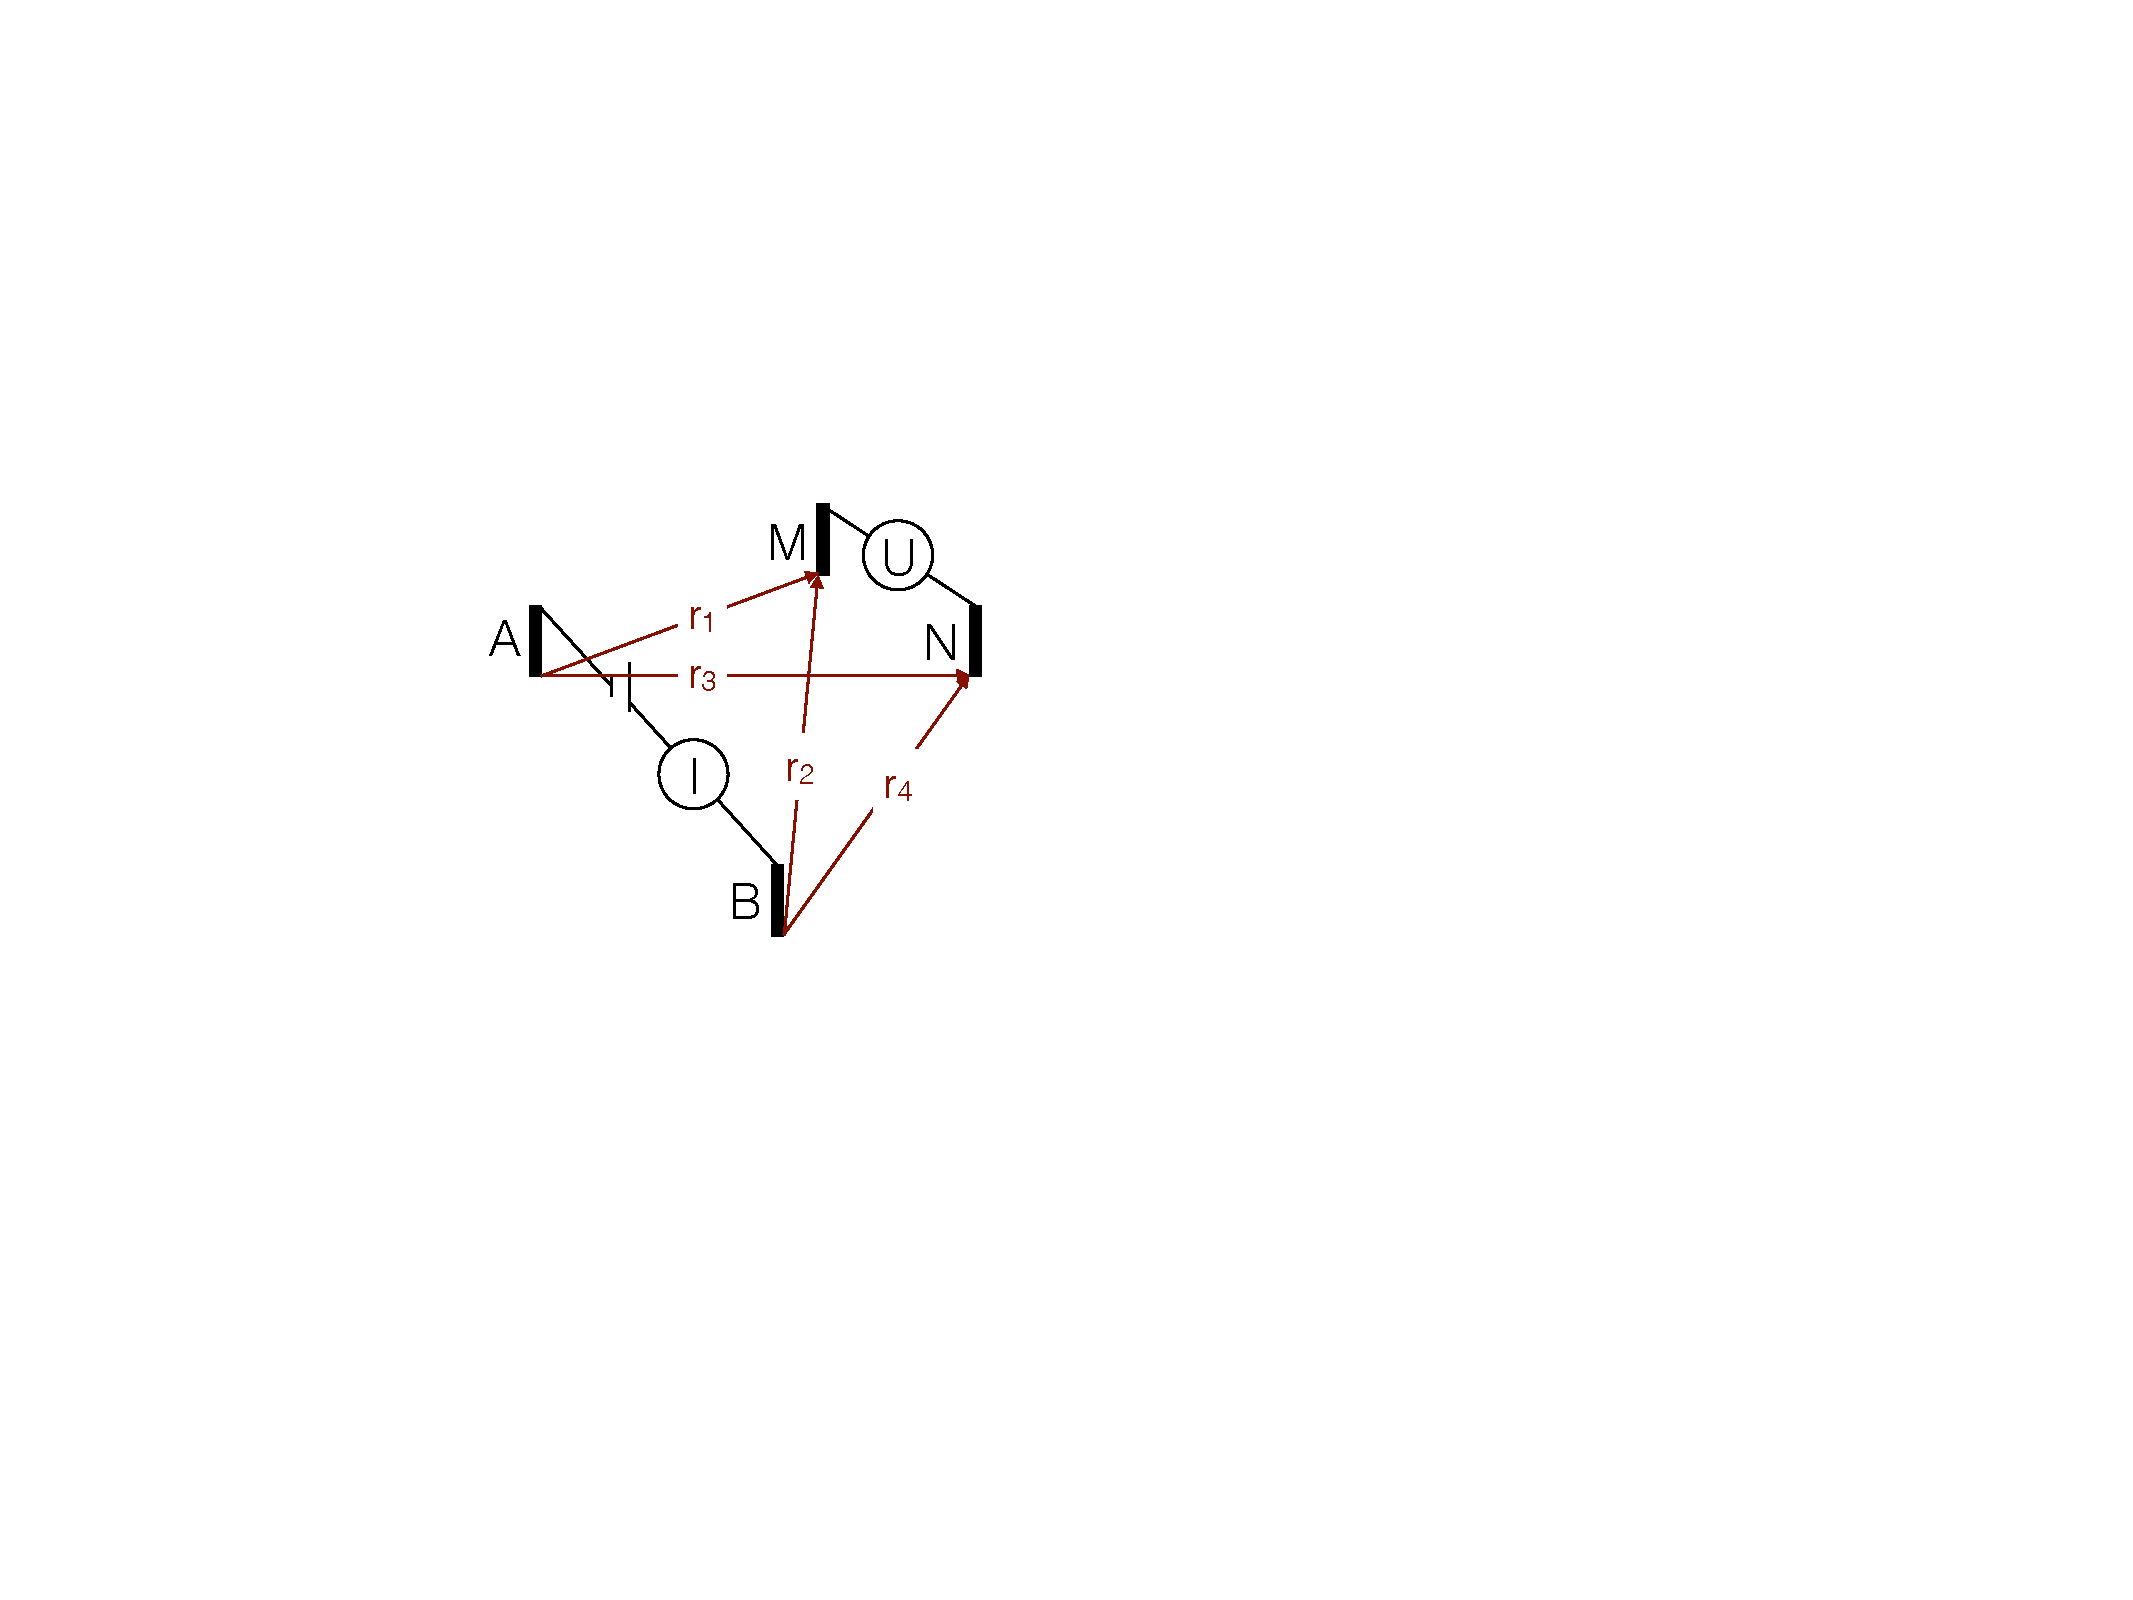
\includegraphics[scale = 0.8]{GeoelektrikBilder/beliebigeVierpunktanordnung}
\end{figure}



\subsection{Sondierung}
Ist eine Untersuchung der Struktur unter einem bestimmten Punkt vorgesehen, eignet sich die \textbf{Schlumberger-Anordnung}.
Bei dieser Messkonfiguration ist der Abstand zwischen den Elektroden A und B deutlich größer als der Abstand zwischen den Sonden M und N. Im Laufe der Messung wird der Abstand von A und B symmetrisch zu N und M immer weiter vergrößert, während N und M am selben Ort bleiben. Durch diese Art der Messung ergeben sich Informationen über den spezifischen Widerstand in immer größeren Tiefen.


\begin{figure}[H]
	\centering
	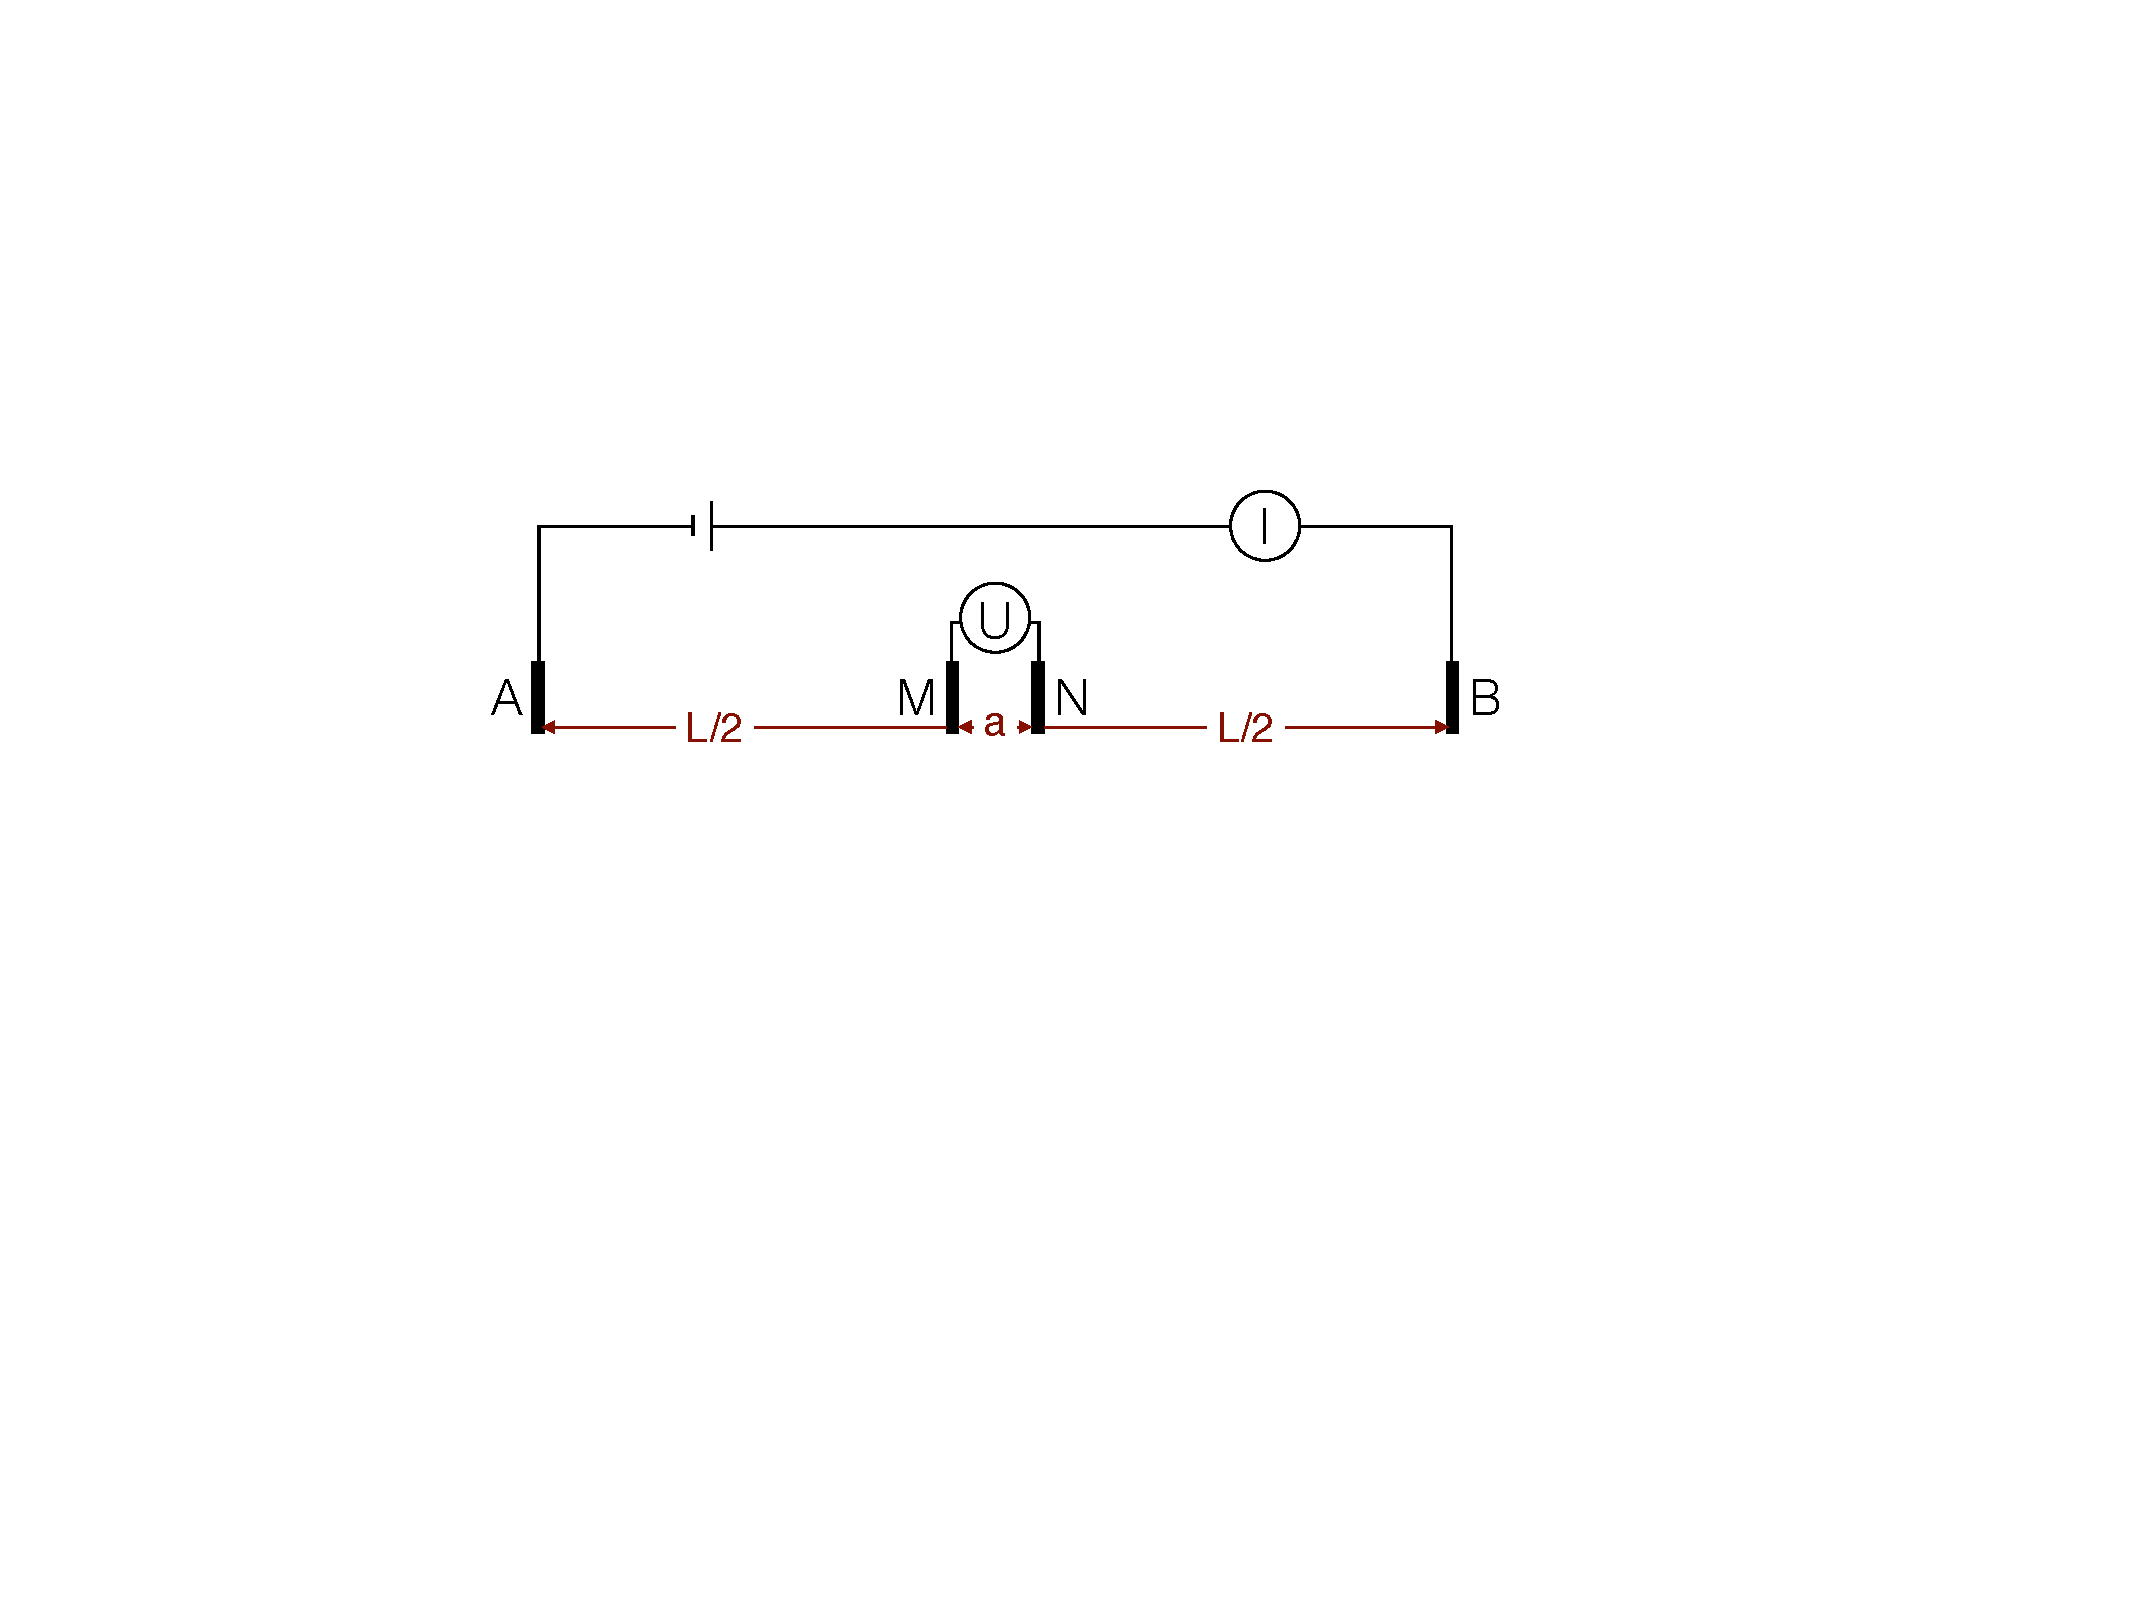
\includegraphics[width = \textwidth]{GeoelektrikBilder/SchlumbergerAnordnung}
\end{figure}


\subsection{Kartierung}
Von einer Kartierung spricht man dann, wenn die Struktur in einer bestimmten Tiefe flächenhaft untersucht werden soll. Hierfür findet die \textbf{Wenner-Anordnung} Verwendung. Im Vergleich zur Schlumberger-Anordnung ist hier der Abstand aller Elektroden und Sonden gleich. Im Laufe der Messung wird die gesamte Messauslage mit festem Abstand entlang des zu untersuchenden Profils bewegt. Der Elektrodenabstand entspricht etwa der Eindringtiefe.


\begin{figure}[H]
	\centering
	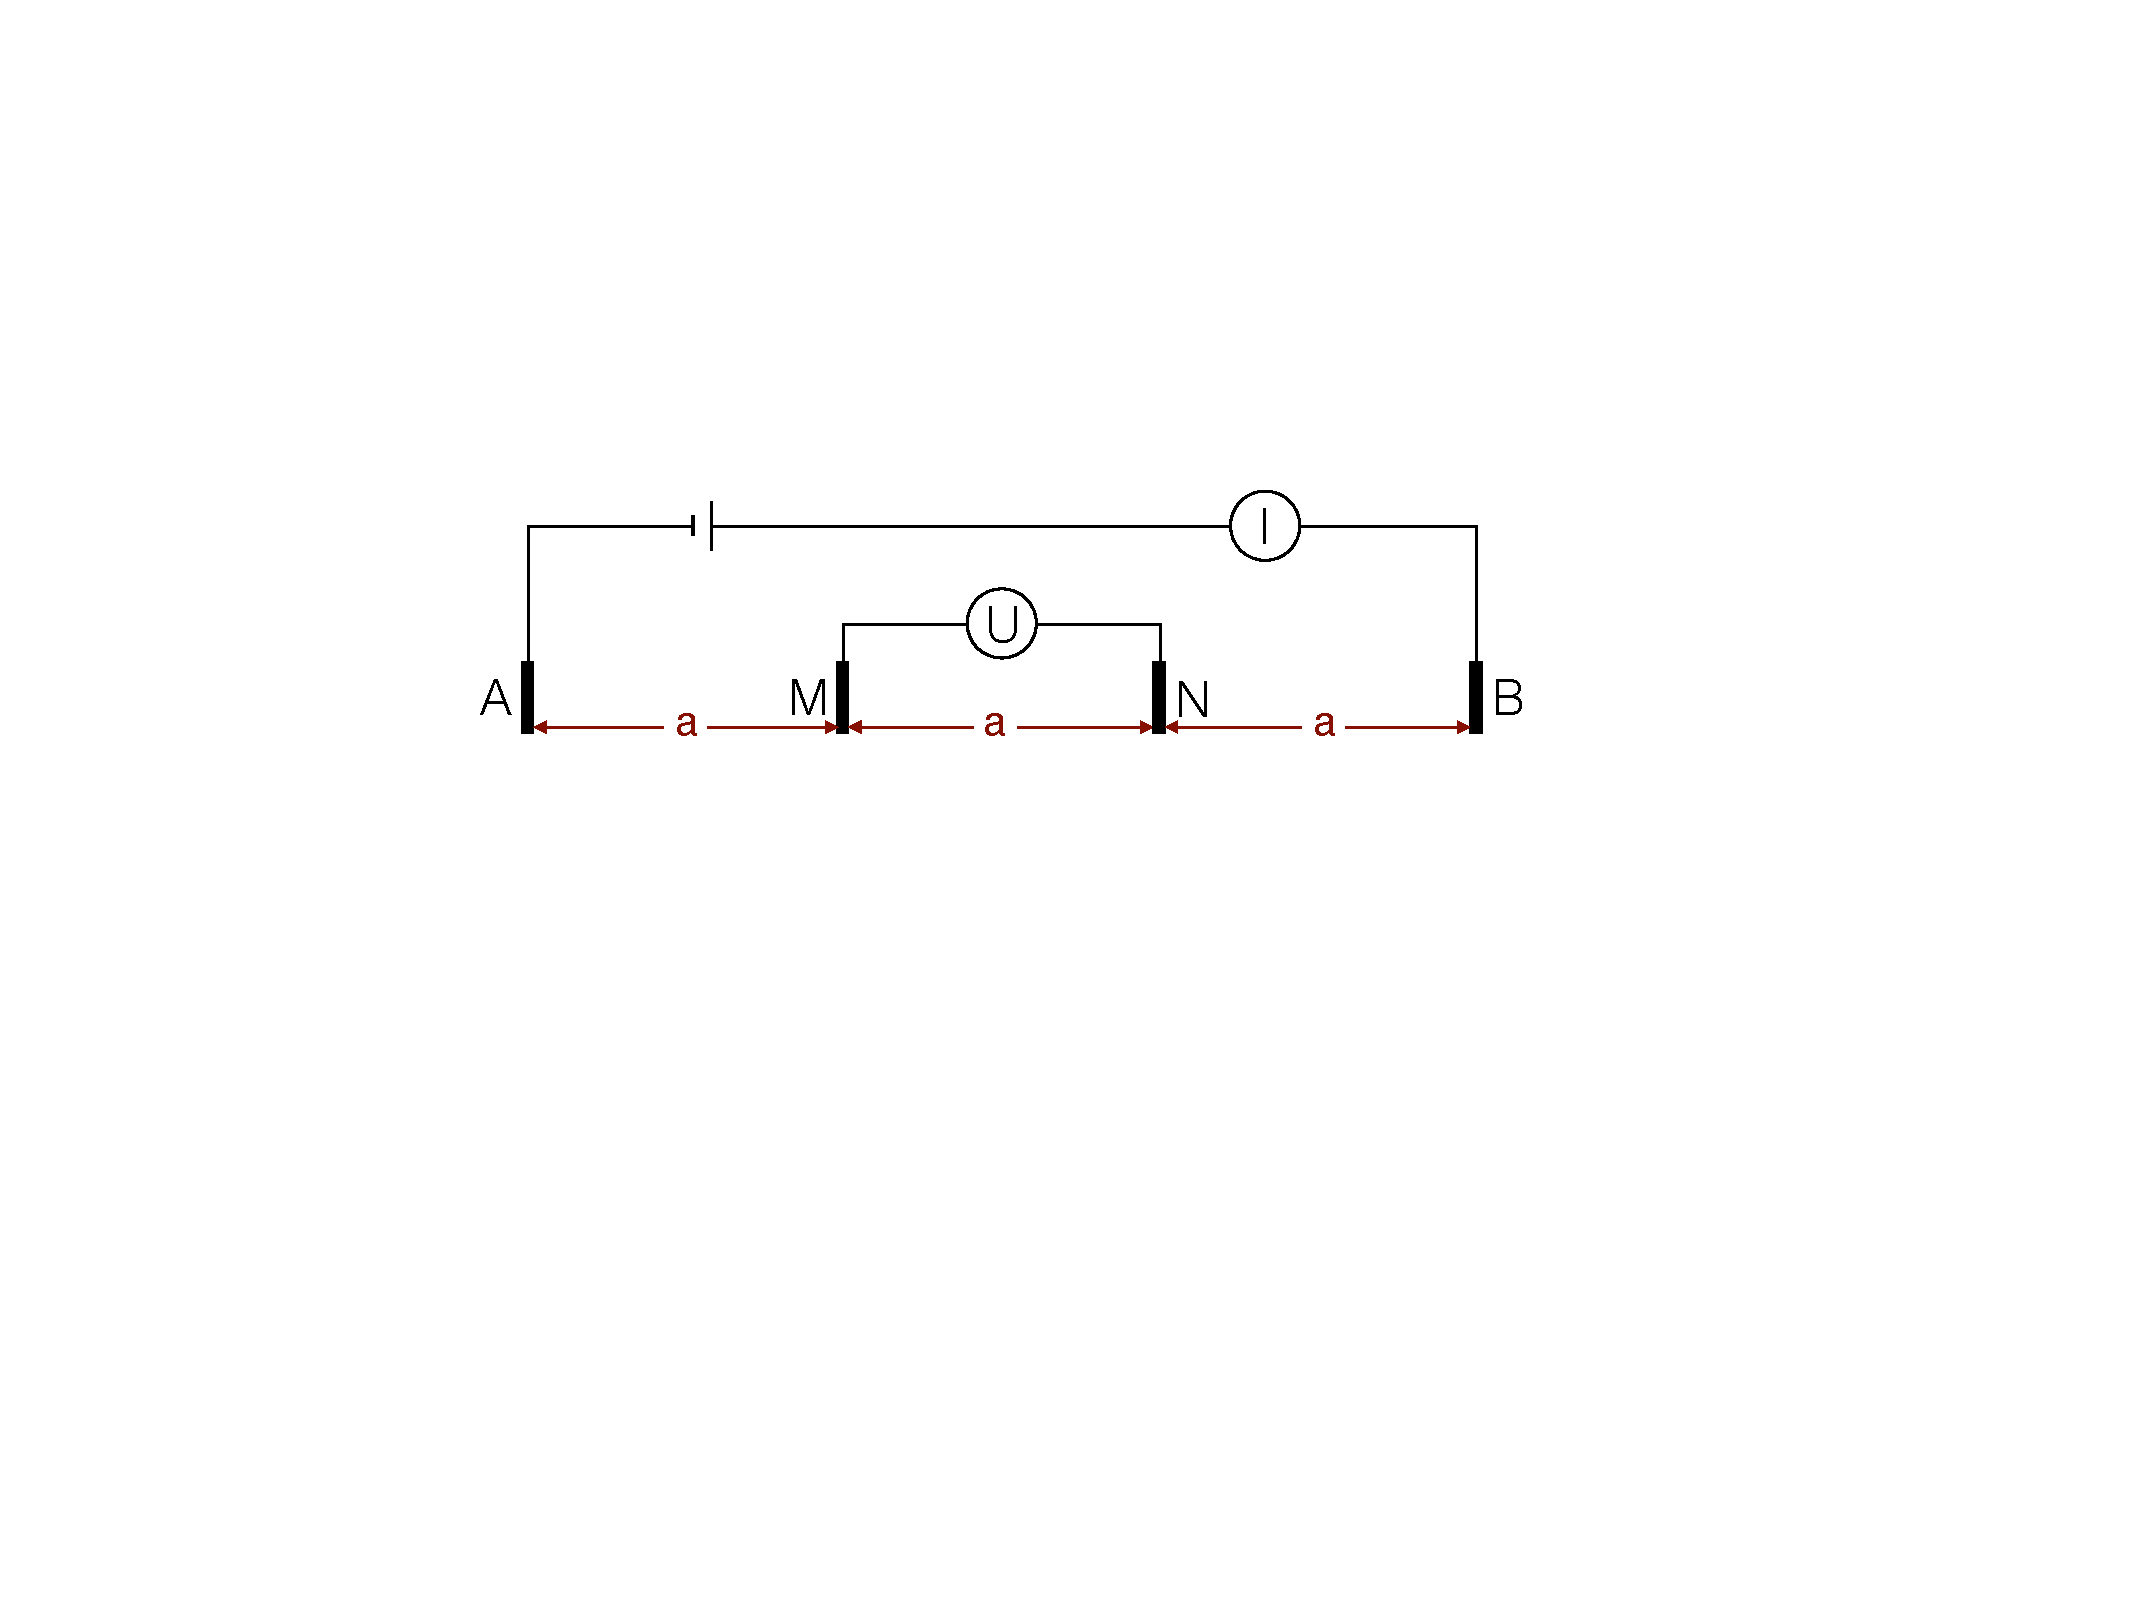
\includegraphics[width = \textwidth]{GeoelektrikBilder/WennerAnordnung}
\end{figure}



\subsection{Dipol-Dipol-Anordnung}
Diese Anordnung trennt Spannungsmessung und Stromzufuhr. Die Elektroden A und B zur Stromeinspeisung haben dabei den selben Abstand $a$ wie die Sonden N und M zur Spannungsmessung. Der Abstand dieser beiden Paare ist ein Vielfaches von $a$.

\begin{figure}[H]
	\centering
	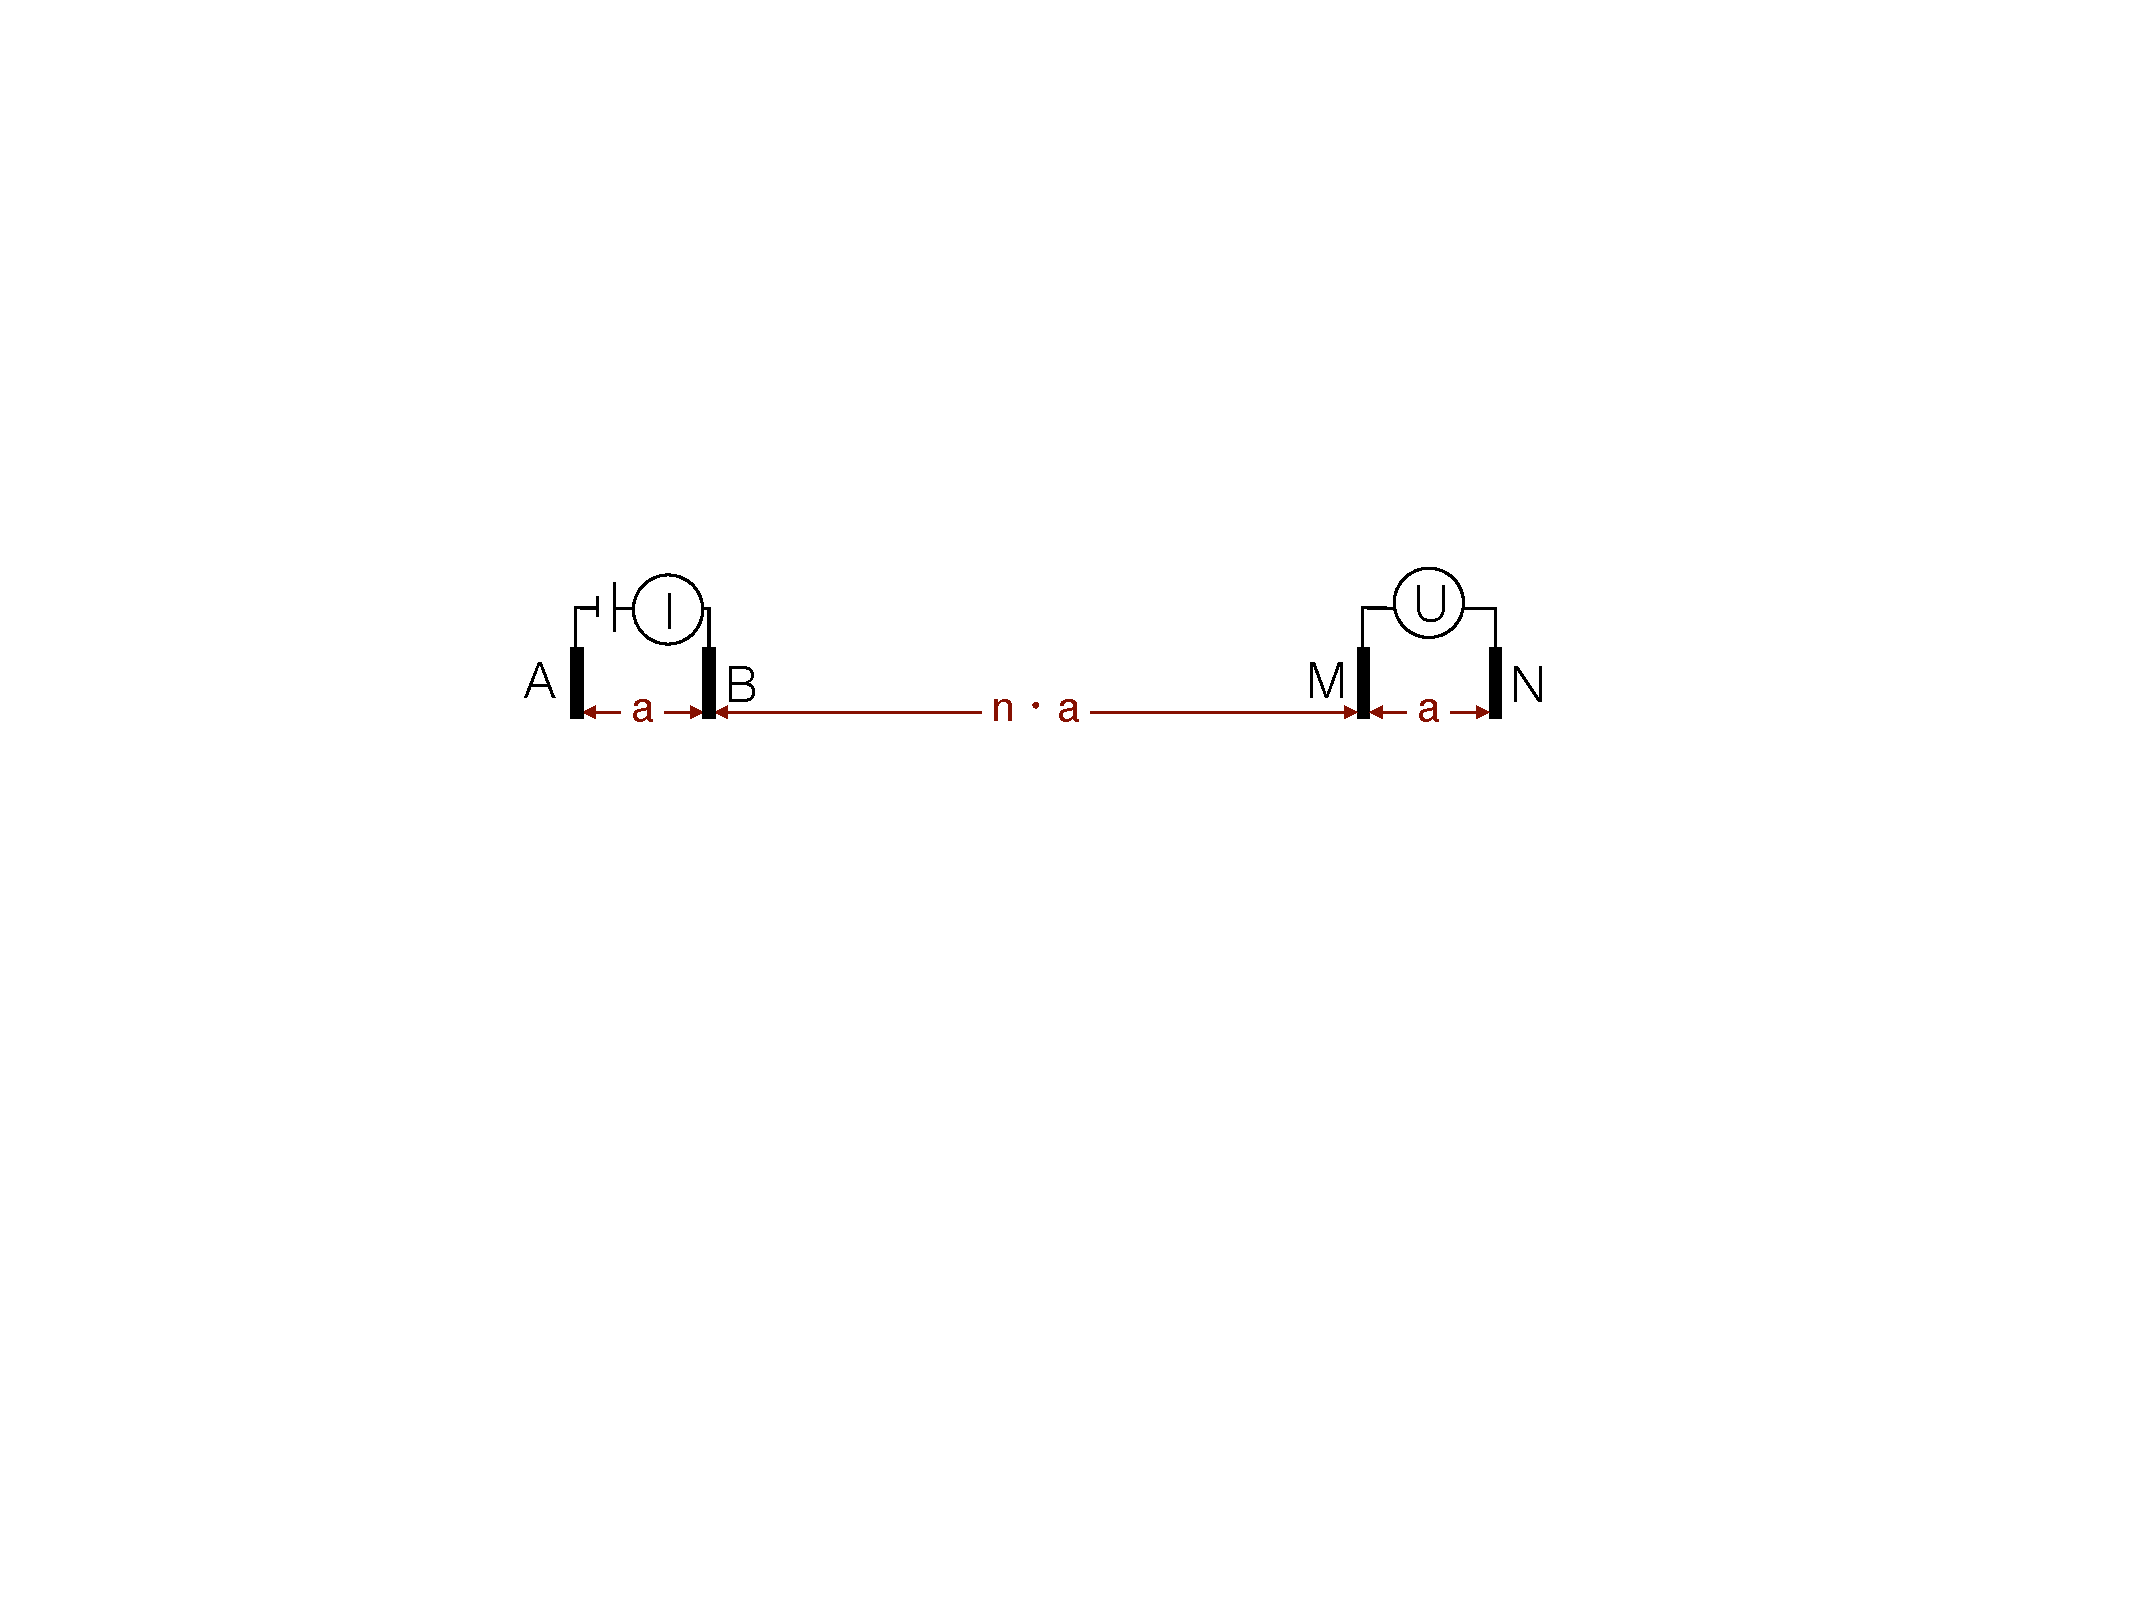
\includegraphics[width = \textwidth]{GeoelektrikBilder/DipolDipolAnordnung}
\end{figure}


\section{Auswertung}
Um Rückschlüsse auf die Beschaffenheit des Untergrundes ziehen zu können, muss der scheinbare spezifische Widerstand $\rho_{\text{s}}$ berechnet werden. 
Bei Gleichstromverfahren ist das relativ einfach. Der scheinbare spezifische Widerstand berechnet sich zu \begin{equation*}
	\rho_{\text{s}} = R \cdot K = \frac{U}{I} \cdot K
\end{equation*}

$K$ bezeichnet hierbei den Geometriefaktor der verwendeten Anordnung.

Verändert sich der scheinbare spezifische Widerstand im Laufe einer Messung kaum oder nicht, spricht man vom Medium des Untergrundes als homogenen Halbraum. 

Für die Auswertung des spezifischen Widerstandes gibt es gewissen Anhaltspunkte. In Mineralen ist der spezifische Widerstand groß und in Metallen, Erzen oder Graphit klein. \\
Eine Diskontinuität im Untergrund kenntzeichnet sich durch eine deutliche Veränderung des spezifischen Widerstandes. Solche signifikanten Änderungen werden beispielsweise durch Wasser, Salze oder Metalle und Erze hervorgerufen. Um ein Gefühl für die Größenunterschiede zu bekommen, seien nun noch ein paar Literaturwerte genannt. 

\begin{tabular}{ll}
	\textbf{Gestein} & \textbf{spezifischer Widerstand [$\Omega$m]} \\
	Sand (trocken) & $10^5$ \\
	Sand (wassergesättigt) & 1000 -- $10^4$ \\
	Granit & 300 - $3 \cdot 10^4$ \\
	Kalkstein & 100 -- 7000 \\
	Lehme & 3 -- 300 \\
	Ton (trocken) & 30 -- 1000 \\
	Ton (nass) & 1-30
\end{tabular}  

\subsection{Geometriefaktor}
Dieser Faktor ist wichtig, da sich der scheinbare spezifische Widerstand je nach verwendeter Anordnung ändert. Ohne Herleitung seien hier die Geometriefaktoren der vier präsentierten Messkonfigurationen genannt:

\subsubsection{beliebige Vierpunktanordnung}

\begin{figure}[H]
	\begin{subfigure}[m]{0.5\textwidth}
	\centering
		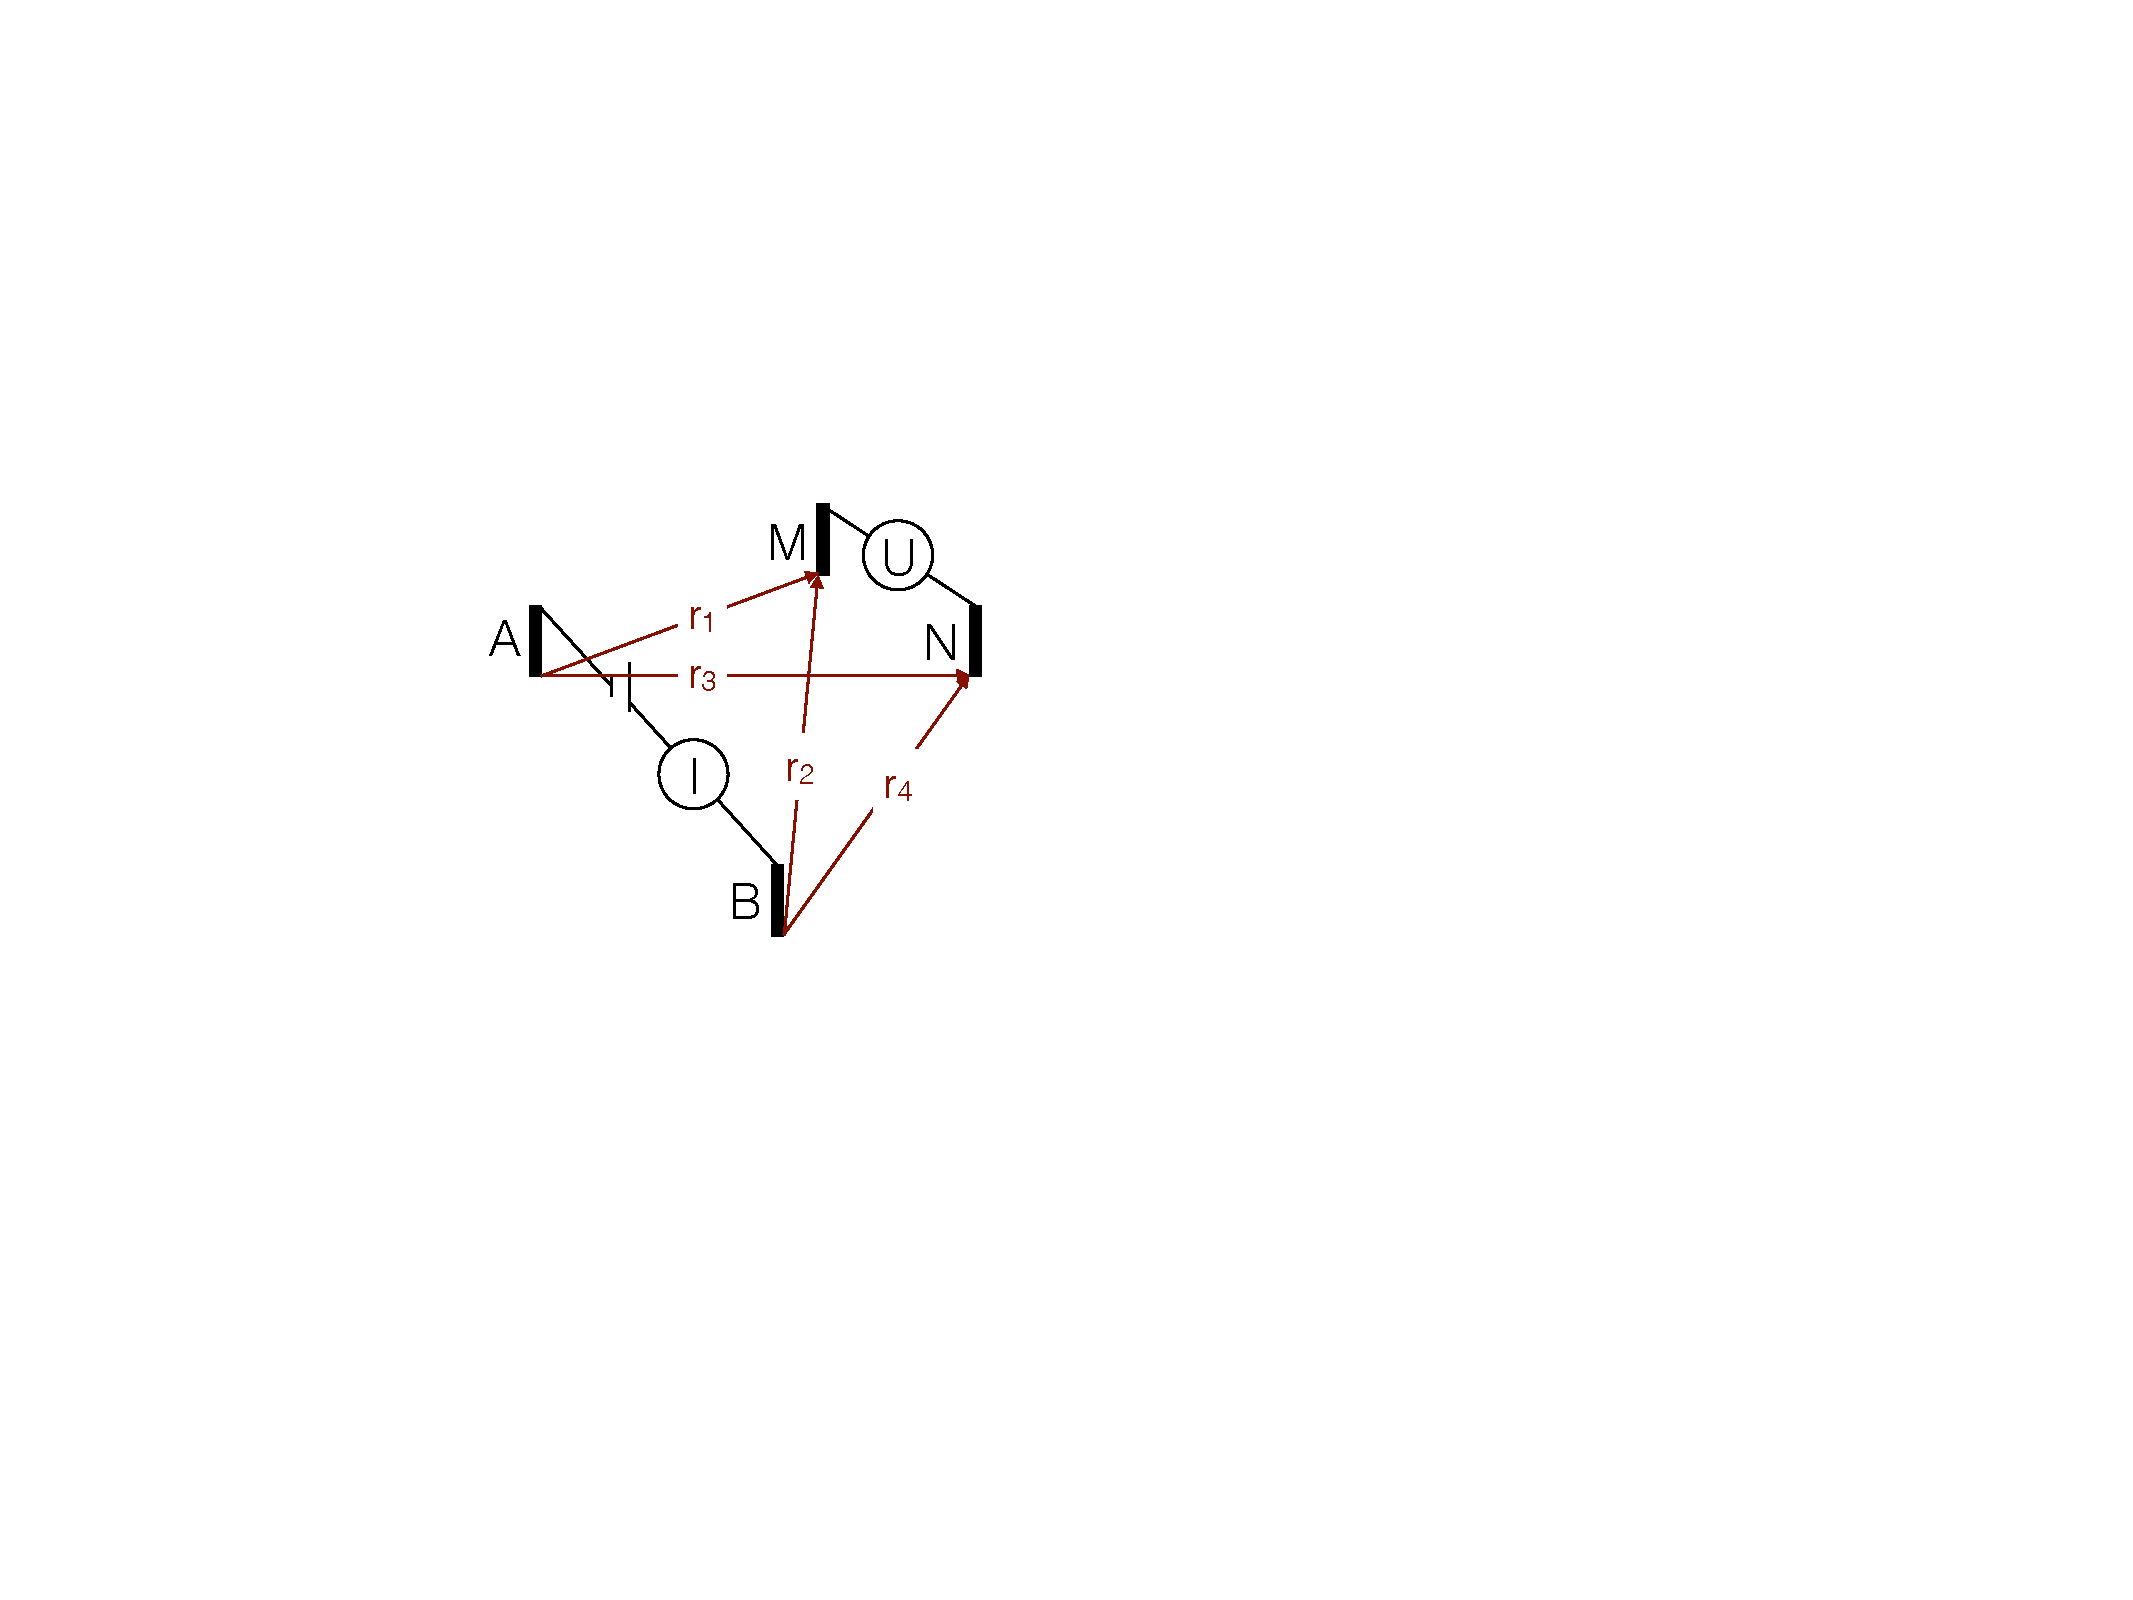
\includegraphics[scale = 0.5]{GeoelektrikBilder/beliebigeVierpunktanordnung}
	\end{subfigure}
	\begin{subfigure}[m]{0.5\textwidth}
		\begin{equation*}
			K = \frac{2 \pi}{\left( \frac{1}{r_1} - \frac{1}{r_2} \right) - \left( \frac{1}{r_3} - \frac{1}{r_4} \right)}
		\end{equation*}
	\end{subfigure}
\end{figure}


\subsubsection{Schlumberger-Anordnung}

\begin{figure}[H]
	\begin{subfigure}[m]{0.5\textwidth}
	\centering
		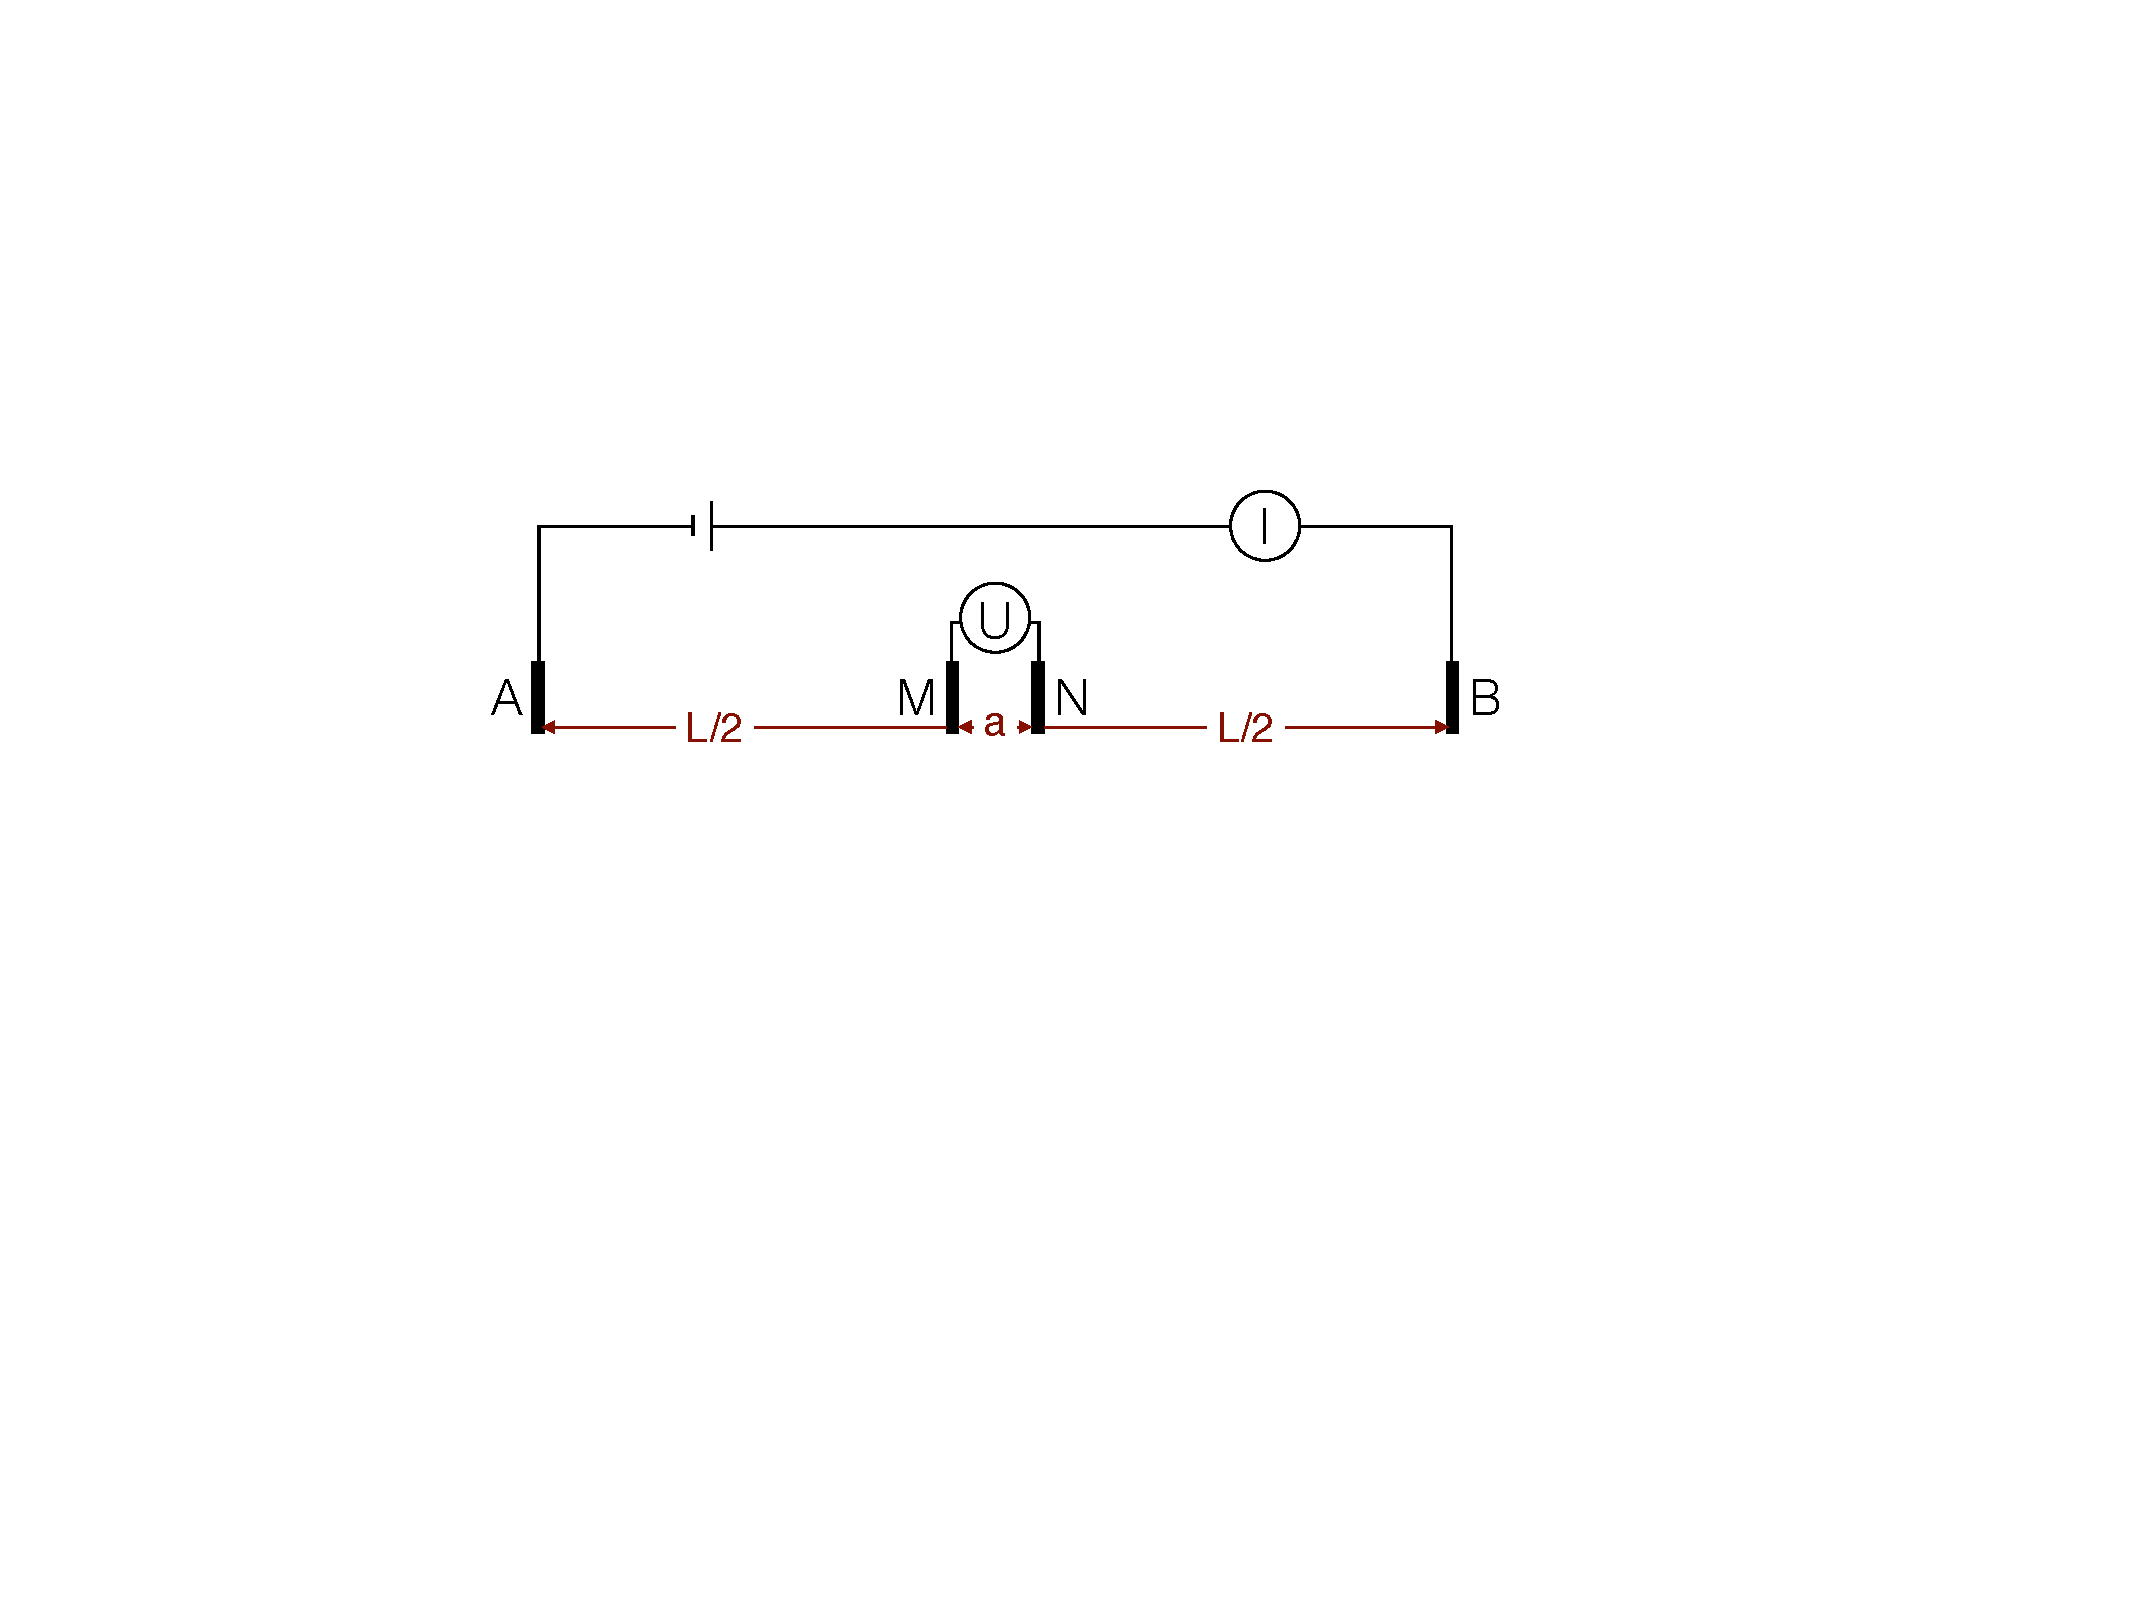
\includegraphics[scale = 0.4]{GeoelektrikBilder/SchlumbergerAnordnung}
	\end{subfigure}
	\begin{subfigure}[m]{0.5\textwidth}
		\begin{equation*}
			K = \frac{\pi}{a} \cdot \left( \frac{L}{2} \right)^2
		\end{equation*}
	\end{subfigure}
\end{figure}


\subsubsection{Wenner-Anordnung}

\begin{figure}[H]
	\begin{subfigure}[m]{0.5\textwidth}
	\centering
		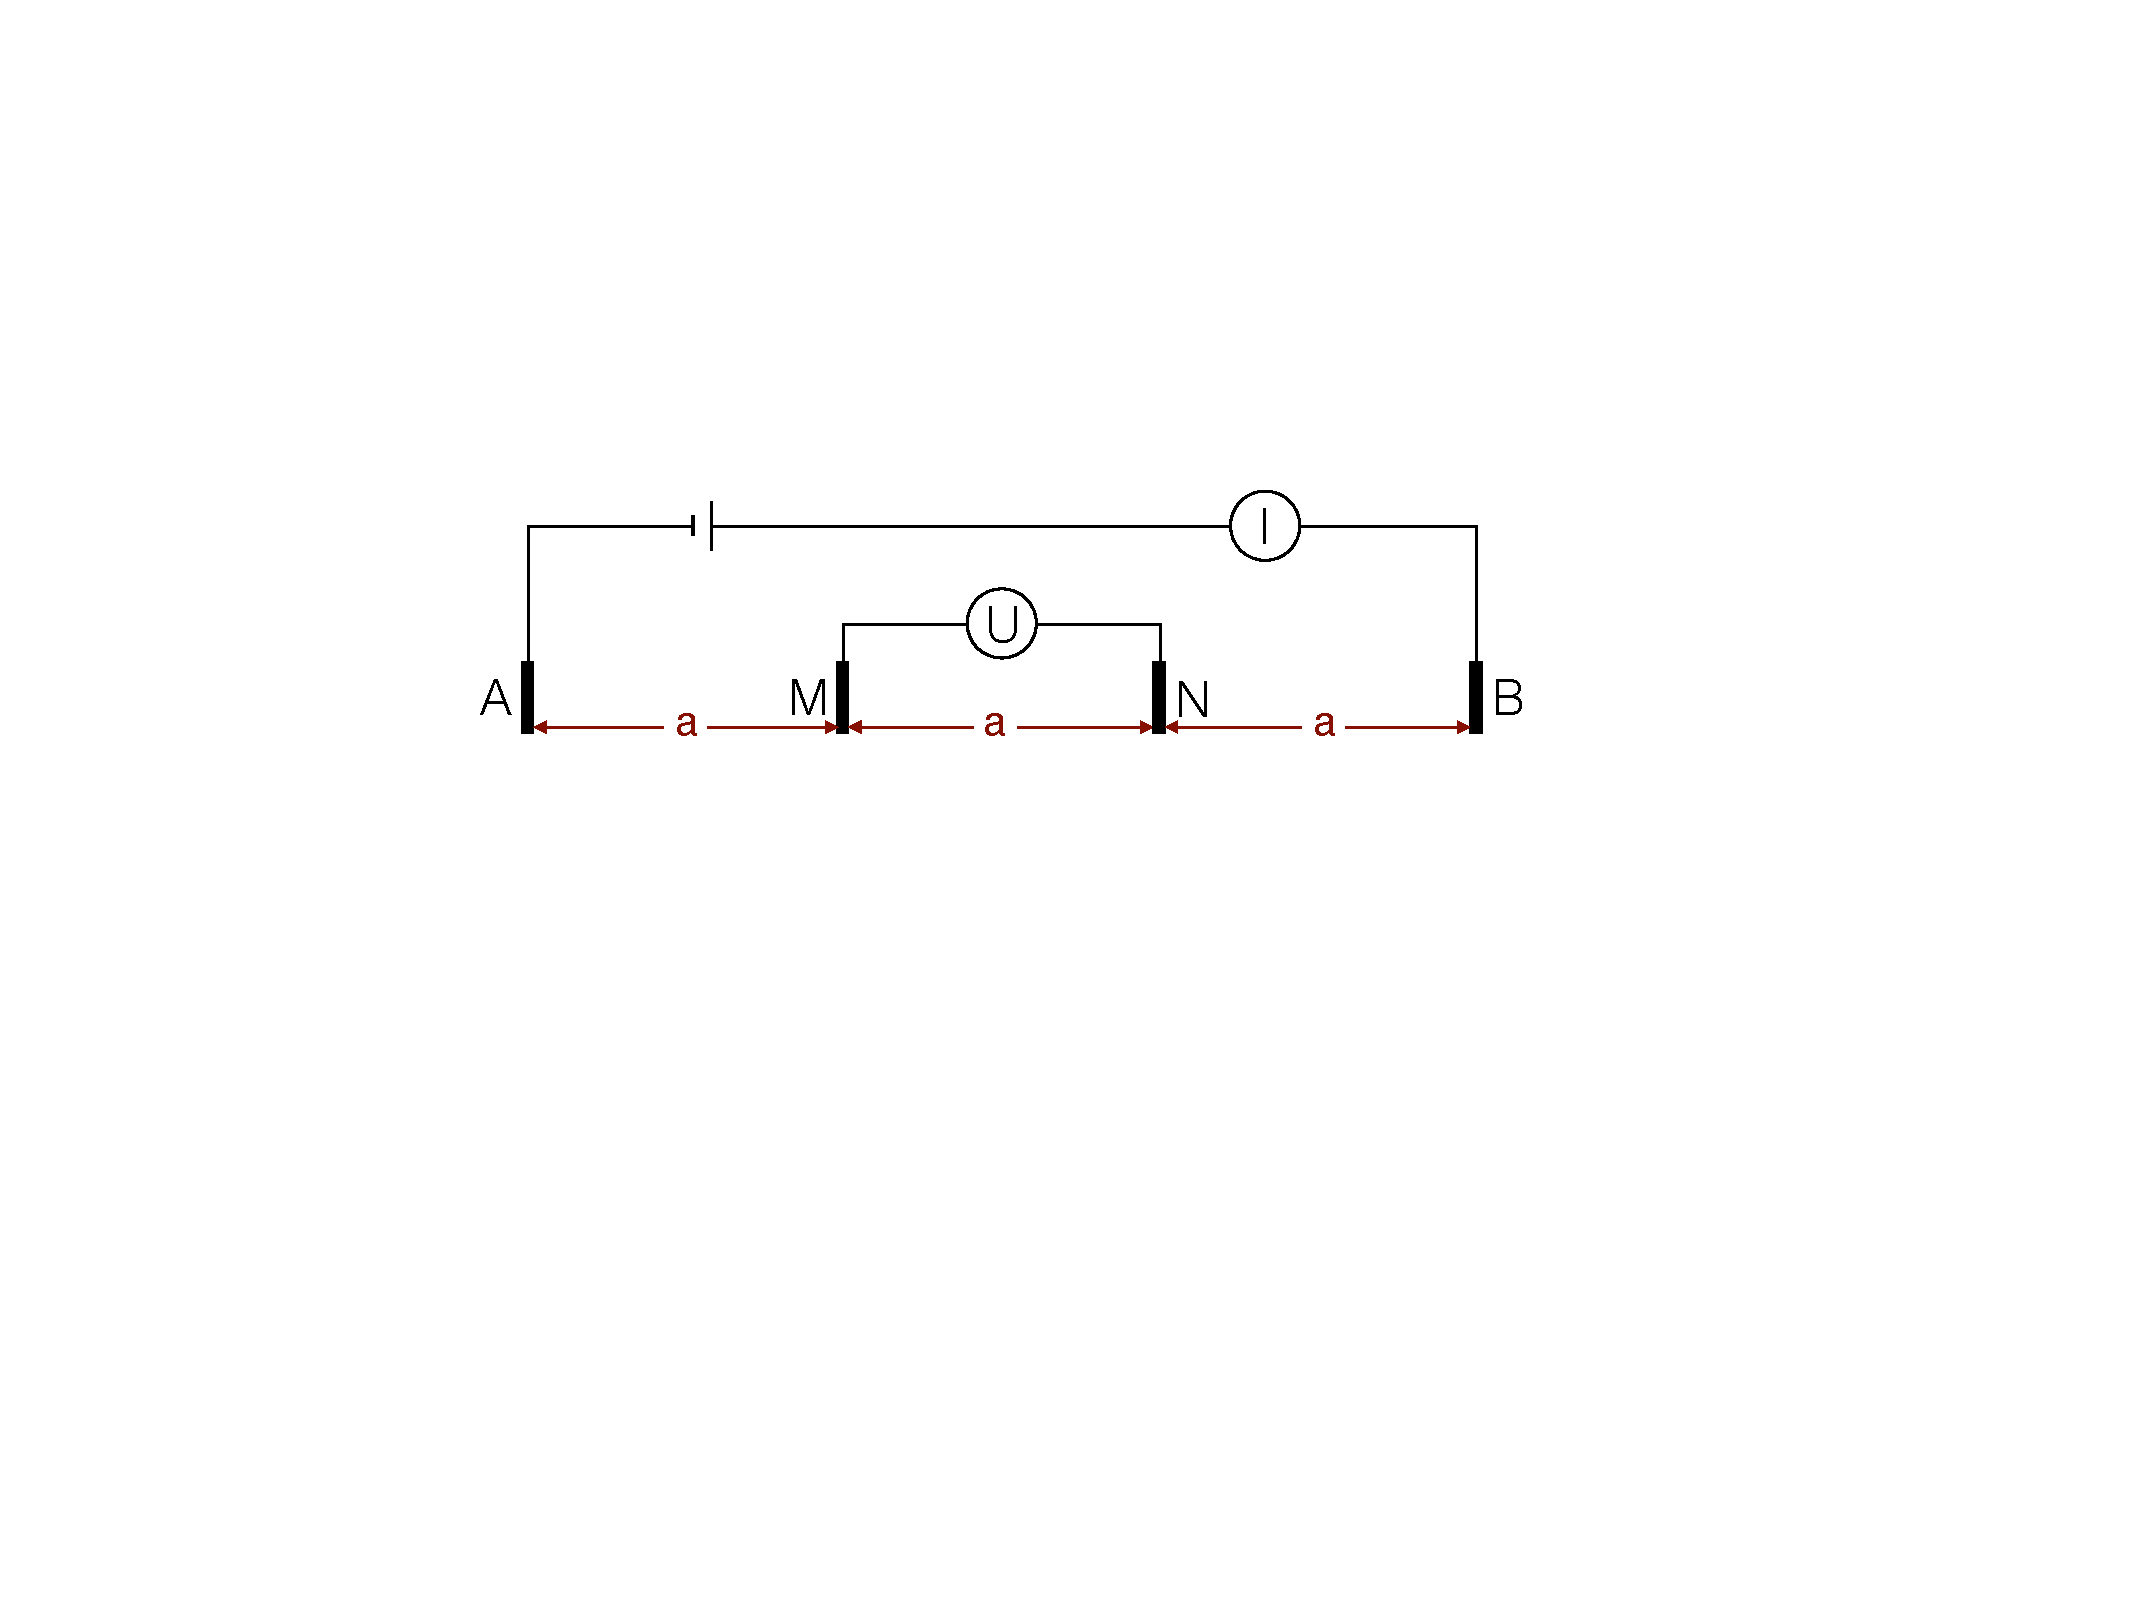
\includegraphics[scale = 0.4]{GeoelektrikBilder/WennerAnordnung}
	\end{subfigure}
	\begin{subfigure}[m]{0.5\textwidth}
		\begin{equation*}
				K = 2 \pi \cdot a
		\end{equation*}
	\end{subfigure}
\end{figure}



\subsubsection{Dipol-Dipol-Anordnung}

\begin{figure}[H]
	\begin{subfigure}[m]{0.5\textwidth}
	\centering
		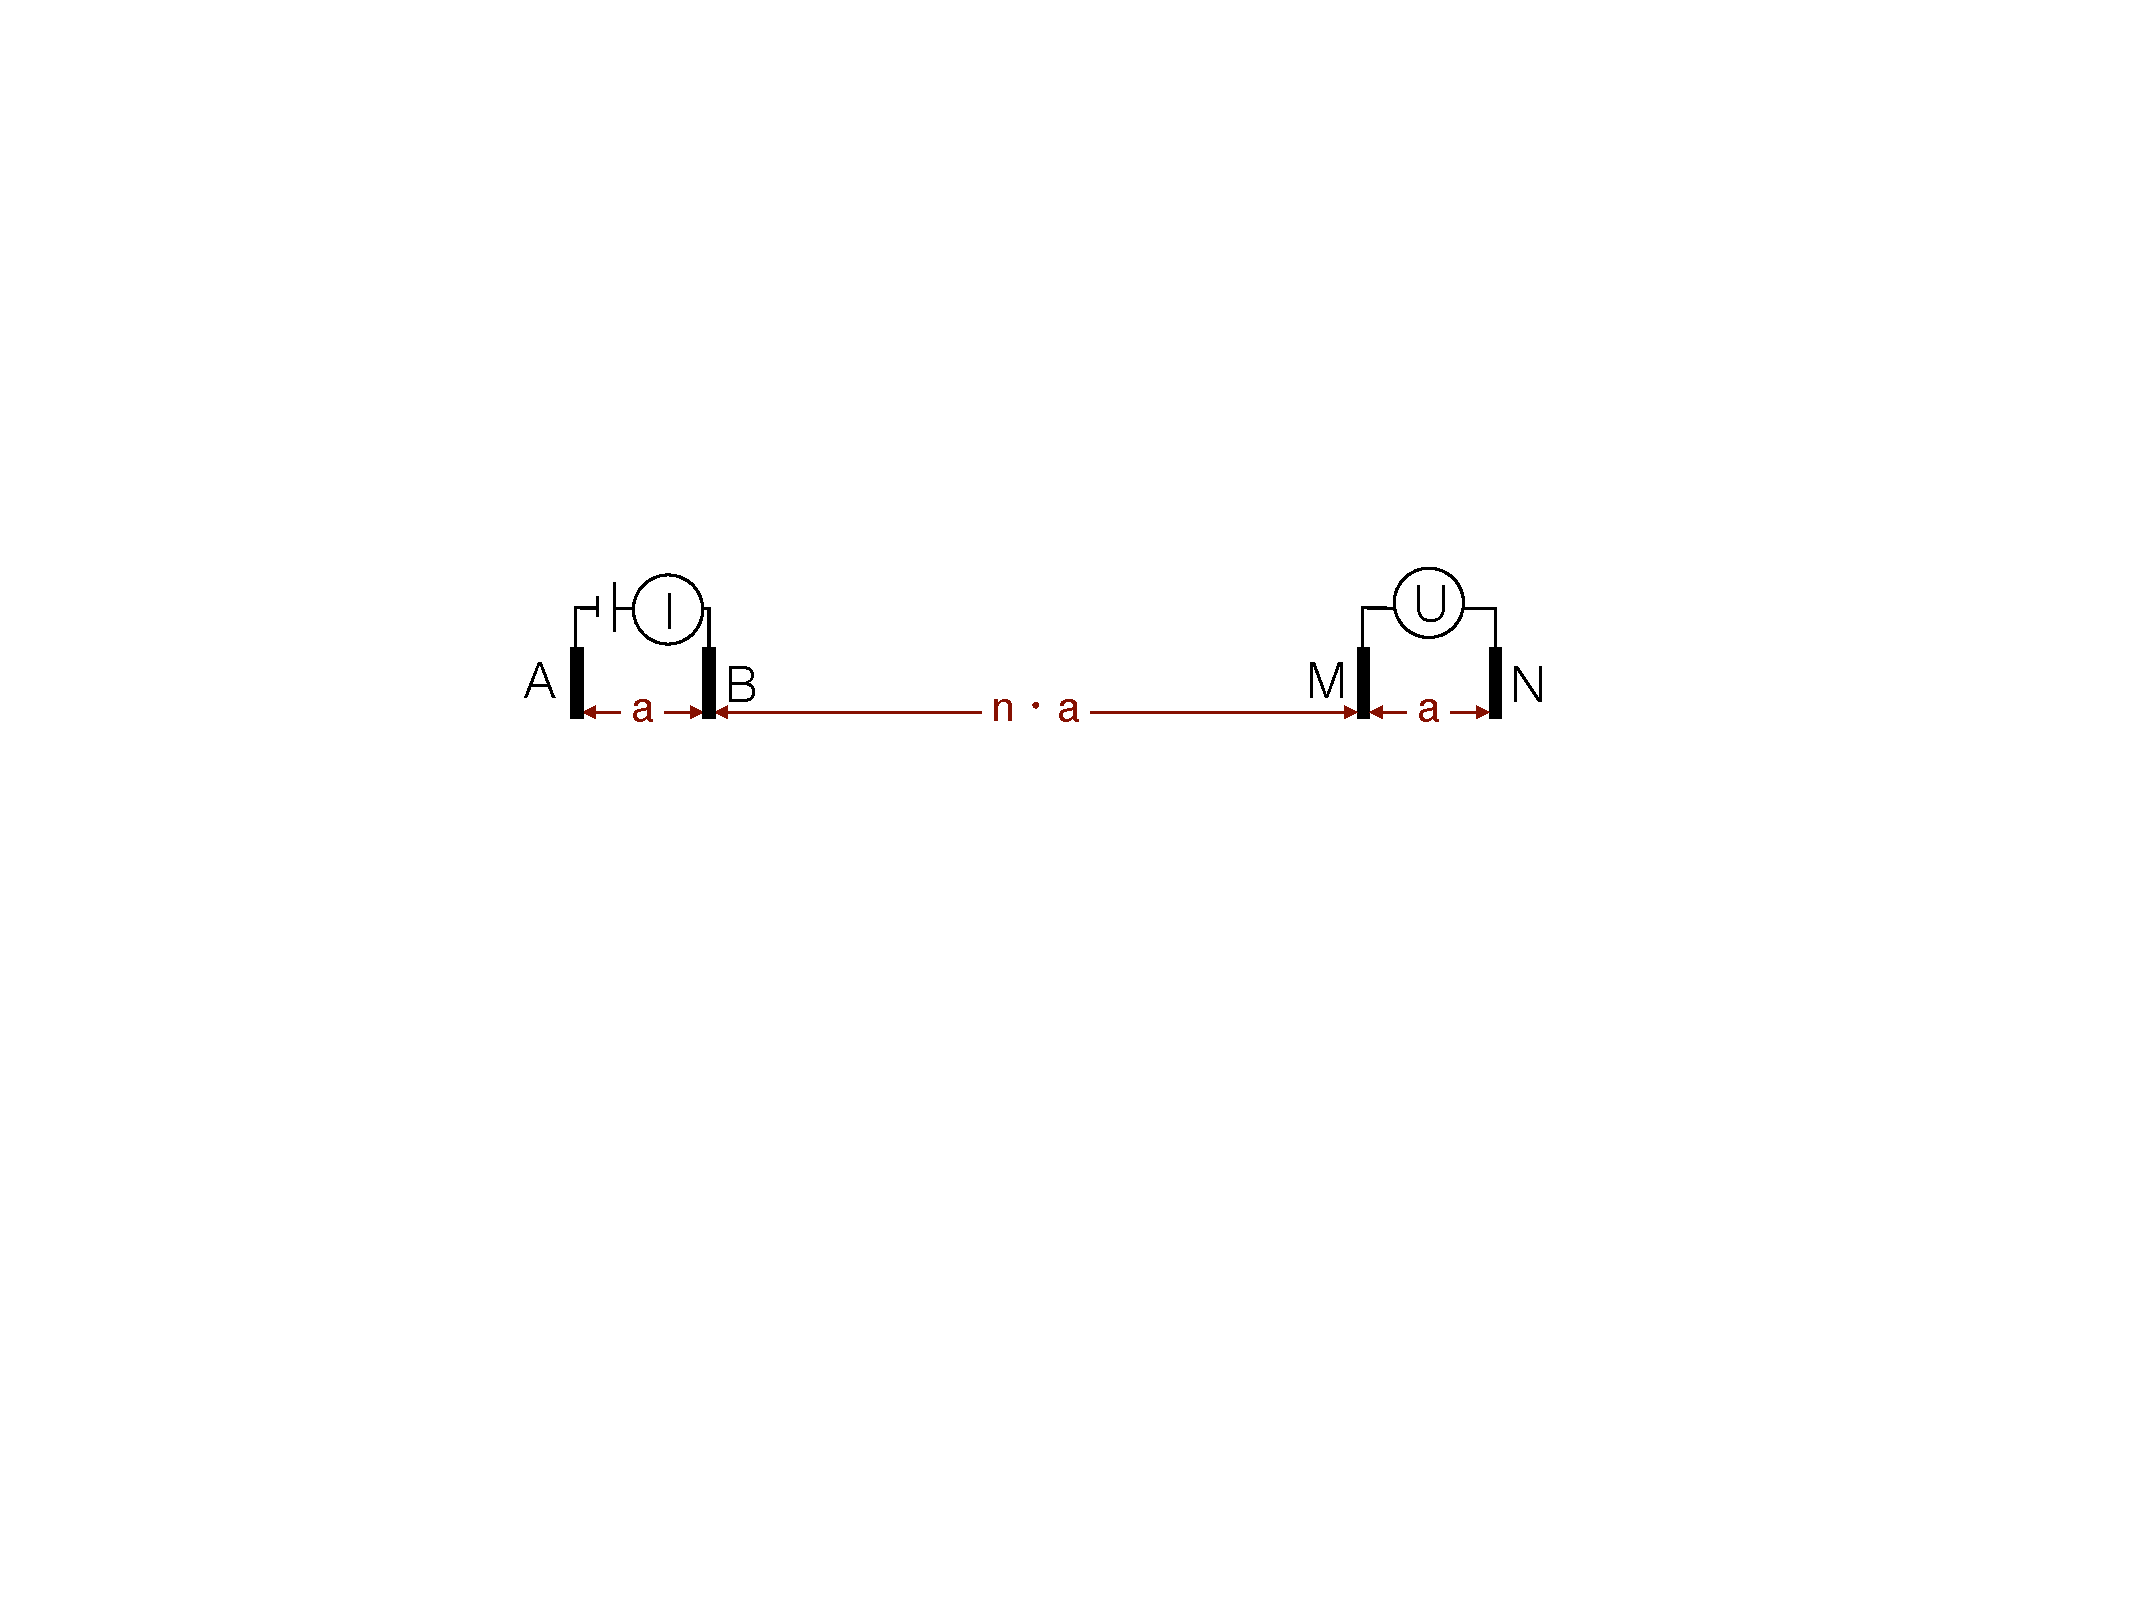
\includegraphics[scale = 0.35]{GeoelektrikBilder/DipolDipolAnordnung}
	\end{subfigure}
	\begin{subfigure}[m]{0.5\textwidth}
		\begin{equation*}
				K = \pi \cdot a \cdot n \cdot (n+1) \cdot (n+2)
		\end{equation*}
	\end{subfigure}
\end{figure}


\subsection{Stromfluss im Halbraum}
Bei einer Messung mit Vierpunktanordnung wird Strom in die Erde eingespeist. Dadurch entsteht ein elektrisches Feld, welches sich durch Feldlinien charakterisieren lässt. Diese Feldlinien sind senkrecht zur Stromrichtung und bilden Äquipotentialflächen, also Flächen, an denen das gleiche Potential anliegt.   

\begin{figure}[H]
	\centering
	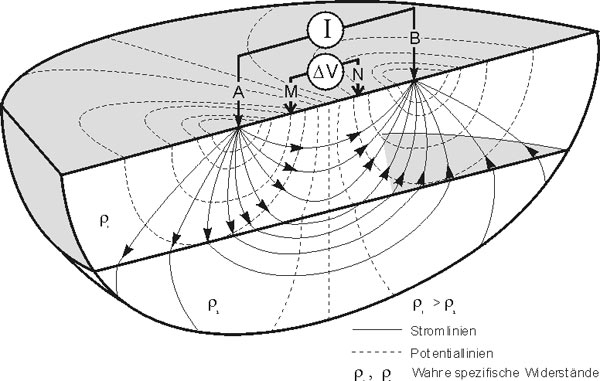
\includegraphics[width = \textwidth]{GeoelektrikBilder/EFeldErde}	
	\caption*{\textsl{Quelle: umwelt.sachsen.de}}
\end{figure}

 




